\documentclass[]{elsarticle} %review=doublespace preprint=single 5p=2 column
%%% Begin My package additions %%%%%%%%%%%%%%%%%%%
\usepackage[hyphens]{url}

  \journal{Transportation Findings} % Sets Journal name


\usepackage{lineno} % add
\providecommand{\tightlist}{%
  \setlength{\itemsep}{0pt}\setlength{\parskip}{0pt}}

\usepackage{graphicx}
\usepackage{booktabs} % book-quality tables
%%%%%%%%%%%%%%%% end my additions to header

\usepackage[T1]{fontenc}
\usepackage{lmodern}
\usepackage{amssymb,amsmath}
\usepackage{ifxetex,ifluatex}
\usepackage{fixltx2e} % provides \textsubscript
% use upquote if available, for straight quotes in verbatim environments
\IfFileExists{upquote.sty}{\usepackage{upquote}}{}
\ifnum 0\ifxetex 1\fi\ifluatex 1\fi=0 % if pdftex
  \usepackage[utf8]{inputenc}
\else % if luatex or xelatex
  \usepackage{fontspec}
  \ifxetex
    \usepackage{xltxtra,xunicode}
  \fi
  \defaultfontfeatures{Mapping=tex-text,Scale=MatchLowercase}
  \newcommand{\euro}{€}
\fi
% use microtype if available
\IfFileExists{microtype.sty}{\usepackage{microtype}}{}
\bibliographystyle{elsarticle-harv}
\usepackage{graphicx}
% We will generate all images so they have a width \maxwidth. This means
% that they will get their normal width if they fit onto the page, but
% are scaled down if they would overflow the margins.
\makeatletter
\def\maxwidth{\ifdim\Gin@nat@width>\linewidth\linewidth
\else\Gin@nat@width\fi}
\makeatother
\let\Oldincludegraphics\includegraphics
\renewcommand{\includegraphics}[1]{\Oldincludegraphics[width=\maxwidth]{#1}}
\ifxetex
  \usepackage[setpagesize=false, % page size defined by xetex
              unicode=false, % unicode breaks when used with xetex
              xetex]{hyperref}
\else
  \usepackage[unicode=true]{hyperref}
\fi
\hypersetup{breaklinks=true,
            bookmarks=true,
            pdfauthor={},
            pdftitle={Using Google Community Mobility Reports to investigate the growth of COVID-19 in the United States},
            colorlinks=false,
            urlcolor=blue,
            linkcolor=magenta,
            pdfborder={0 0 0}}
\urlstyle{same}  % don't use monospace font for urls

\setcounter{secnumdepth}{0}
% Pandoc toggle for numbering sections (defaults to be off)
\setcounter{secnumdepth}{0}


% Pandoc header
\usepackage{booktabs}
\usepackage{longtable}
\usepackage{array}
\usepackage{multirow}
\usepackage{wrapfig}
\usepackage{float}
\usepackage{colortbl}
\usepackage{pdflscape}
\usepackage{tabu}
\usepackage{threeparttable}
\usepackage{threeparttablex}
\usepackage[normalem]{ulem}
\usepackage{makecell}
\usepackage{xcolor}



\begin{document}
\begin{frontmatter}

  \title{Using Google Community Mobility Reports to investigate the growth of
COVID-19 in the United States}
    \author[McMaster University]{Antonio Paez\corref{1}}
   \ead{paezha@mcmaster.ca} 
      \address[McMaster University]{School of Geography and Earth Sciences, McMaster University, Hamilton,
ON, L8S 4K1, Canada}
      \cortext[1]{Corresponding Author}
  
  \begin{abstract}
  In 2020 Google released a set of Community Mobility Reports (GCMR).
  These reports are based on the company's location-tracking capabilities
  and measure changes in mobility with respect to a baseline. This novel
  source of data offers an opportunity to investigate potential
  correlations between mobility and transmission of COVID-19. Using data
  from the New York Times on COVID-19 cases and GCMR, this paper presents
  an analysis of mobility levels and new daily reported cases of COVID-19
  by state in the US. The results provide insights about the utility and
  interpretability of GCMR for COVID-19 research and decision-making.
  \end{abstract}
  
 \end{frontmatter}

\hypertarget{research-questions-and-hypotheses}{%
\section{Research Questions and
Hypotheses}\label{research-questions-and-hypotheses}}

The main policy tool to control the spread of the COVID-19 pandemic has
been stay-at-home orders, which in the United States have been
implemented on a state-by-state basis, with considerable variations in
compliance. Concurrently, numerous initiatives have been developed to
track the progress and the impact of the pandemic. As a result, there
are new sources of data such as the recently-released Google Community
Mobility Reports
(GCMR)\footnote{https://www.google.com/covid19/mobility/}, as well as
The New York Times repository of COVID-19
data\footnote{https://github.com/nytimes/covid-19-data}. These two open
data sets offer novel opportunities to investigate in quasi-real time
the relationship between mobility patterns and transmission of COVID-19.

This paper investigates the potential of Google Community Mobility
Reports to asses the impact of mobility on COVID-19. The following
questions are posed:

\begin{itemize}
\tightlist
\item
  Do changes in mobility according to GCMR correlate with the
  transmission of COVID-19?
\item
  And if so, what do we learn about mobility and the spread of the
  disease?
\end{itemize}

This paper is a reproducible research document. The source is an
\texttt{R} markdown file available in a public
repository\footnote{See folder Covid-19-Google-CMR-US in \url{https://github.com/paezha/Google-Mobility-Reports-and-COVID-19-US/}}.

\hypertarget{methods-and-data}{%
\section{Methods and Data}\label{methods-and-data}}

GCMR use aggregated and anonymized data to chart changes in mobility
with respect to different classes of places (see Table
\ref{tab:descriptive-statistics}). Mobility indicators are calculated
based on the frequency and length of visits. The reports give percentage
change from a baseline level, which corresponds to the median value of
mobility of identical days of the week during the period between January
3 and Feb 6, 2020. Covid-19 data is compiled by The New York Times based
on reports from state and local health agencies.

\begin{table}[H]

\caption{\label{tab:descriptive-statistics}\label{tab:descriptive-statistics}Descriptive statistics of the data set}
\centering
\resizebox{\linewidth}{!}{
\fontsize{7}{9}\selectfont
\begin{tabular}[t]{l>{\raggedright\arraybackslash}p{12em}llll}
\toprule
Variable & Definition & min & median & max & sd\\
\midrule
\rowcolor{gray!6}  New Cases & New Daily Cases of COVID-19 & 0 & 90 & 12312 & 1051.67\\
date & Date & 2020-02-27 & 2020-04-04 & 2020-05-02 & \\
\rowcolor{gray!6}  retail & Mobility trends for places like restaurants, cafes, shopping centers, theme parks, museums, libraries, and movie theaters & 0.34 & 0.66 & 1.16 & 0.21\\
groceries & Mobility trends for places like grocery markets, food warehouses, farmers markets, specialty food shops, drug stores, and pharmacies & 0.66 & 0.94 & 1.26 & 0.13\\
\rowcolor{gray!6}  parks & Mobility trends for places like local parks, national parks, public beaches, marinas, dog parks, plazas, and public gardens & 0.36 & 1.15 & 2.1 & 0.26\\
\addlinespace
transit & Mobility trends for places like public transport hubs such as subway, bus, and train stations & 0.24 & 0.72 & 1.14 & 0.23\\
\rowcolor{gray!6}  work & Mobility trends for places of work & 0.34 & 0.63 & 1.07 & 0.2\\
residential & Mobility trends for places of residence & 0.97 & 1.14 & 1.27 & 0.08\\
\bottomrule
\multicolumn{6}{l}{\textit{Note: }}\\
\multicolumn{6}{l}{All mobility indicators are lagged 11-day moving averages}\\
\end{tabular}}
\end{table}

For analysis, all mobility indicators are centered so that the value of
1 is the base mobility, and a 0.01 deviation corresponds to a 1\%
change. The incubation time of the disease is between 2 and 12 days
(95\% interval; see Lauer et al., 2020). Given this, it is to be
expected that any changes in mobility will have a lagged effect (if any)
on the discovery of new cases. For this reason, lagged moving averages
of the mobility indicators are calculated. Furthermore, it is possible
that mobility and reports of new cases of COVID-19 are endogenous, if
the public adjust their mobility according to reports of the incidence.
Therefore, in addition to being consistent with an incubation period,
use of lagged indicators also helps to break this potential endogeneity.

The lagged indicators are calculated as the mean of the mobility
indicator using the values from date-minus-12-days to date-minus-2-days.
Furthermore, using the cumulative number of reported COVID-19 cases, the
total number of new daily cases is calculated. This variable
(log-transformed after adding a small constant) is paired with the
corresponding lagged moving average of the mobility indicators. The
log-transformation is useful to avoid negative values of daily new cases
when making predictions. Table \ref{tab:descriptive-statistics} shows
the descriptive statistics of the data set. Analysis is based on
correlation analysis, multivariate regression, and data visualization.

\hypertarget{findings}{%
\section{Findings}\label{findings}}

Table \ref{tab:correlation-analysis} shows that the mobility indicators
are highly correlated with each other. Two variables are selected for
multivariate analysis: parks- and work-related mobility. Work has a high
correlation with the outcome variable, and its correlation with parks is
relatively weak, which increases the information content of the two
variables. Furthermore, parks- and work-related mobility represent two
dimensions of out-of-home activities: mandatory and discretionary
travel.

\begin{table}[H]

\caption{\label{tab:check-correlations}\label{tab:correlation-analysis}Simple correlation between log(New Cases) and the mobility indicators}
\centering
\resizebox{\linewidth}{!}{
\fontsize{7}{9}\selectfont
\begin{tabular}[t]{lrrrrrrr}
\toprule
  & log\_new\_cases & retail & groceries & parks & transit & work & residential\\
\midrule
\rowcolor{gray!6}  log\_new\_cases & 1.00 & -0.68 & -0.48 & -0.27 & -0.68 & -0.69 & 0.71\\
retail & -0.68 & 1.00 & 0.87 & 0.41 & 0.93 & 0.98 & -0.98\\
\rowcolor{gray!6}  groceries & -0.48 & 0.87 & 1.00 & 0.44 & 0.87 & 0.87 & -0.87\\
parks & -0.27 & 0.41 & 0.44 & 1.00 & 0.49 & 0.39 & -0.41\\
\rowcolor{gray!6}  transit & -0.68 & 0.93 & 0.87 & 0.49 & 1.00 & 0.93 & -0.95\\
\addlinespace
work & -0.69 & 0.98 & 0.87 & 0.39 & 0.93 & 1.00 & -0.99\\
\rowcolor{gray!6}  residential & 0.71 & -0.98 & -0.87 & -0.41 & -0.95 & -0.99 & 1.00\\
\bottomrule
\multicolumn{8}{l}{\textit{Note: }}\\
\multicolumn{8}{l}{All mobility indicators are lagged 11-day moving averages}\\
\end{tabular}}
\end{table}

A regression model is estimated with the log of new daily cases as the
dependent variable. The covariates enter the regression in the form of a
second order polynomial expansion. In addition, the date (centered on
April 5) is introduced to account for the temporal trend of the
pandemic. Finally, an indicator variable for the state of New York and
an interaction with the date are used to distinguish the unusually high
incidence of the disease there. The results appear in Table
\ref{tab:model-results}. The model provides a good fit to the data and
all variables reported are significant at \(p<0.05\) or better.

There is an overall temporal trend that indicates a growing number of
cases over time, at an accelerating rate (see positive sign of
date\^{}2). Mobility related to parks and to work both tend to increase
the number of new cases; the negative sign for their interaction is
indicative of the trade-offs between these two forms of mobility and
their impact on new cases. The influence of parks-related mobility was
relatively weaker early in the pandemic (negative sign of the parks x
date term) but has become more important over time (positive sign of the
parks x date\^{}2 term). The opposite happens with work-related
mobility, which started with a greater effect (positive sign of work x
date term), but whose impact has declined over time (negative sign of
work x date\^{}2 term) New York has on average more new daily cases than
the rest of the states, but this has declined over time (see negative
sign of NY x date).

\begin{table}[H]

\caption{\label{tab:model-results}\label{tab:model-results}Results of estimating regression model. Dependent variable is log(New Cases + 0.0001).}
\centering
\fontsize{7}{9}\selectfont
\begin{tabular}[t]{lcc}
\toprule
Variable & Coefficient Estimate & p-value\\
\midrule
\rowcolor{gray!6}  date & 0.1085 & <0.001\\
date\textasciicircum{}2 & 0.0070 & <0.001\\
\rowcolor{gray!6}  parks\textasciicircum{}2 & 2.1756 & <0.001\\
parks & 8.9203 & <0.001\\
\rowcolor{gray!6}  parks x work & -23.6010 & <0.001\\
\addlinespace
work & 6.3156 & 0.0035\\
\rowcolor{gray!6}  work\textasciicircum{}2 & 12.0539 & <0.001\\
parks x date & -0.2133 & <0.001\\
\rowcolor{gray!6}  parks x date\textasciicircum{}2 & 0.0079 & <0.001\\
work x date & 0.1376 & 0.0272\\
\addlinespace
\rowcolor{gray!6}  work x date\textasciicircum{}2 & -0.0238 & <0.001\\
NY & 3.5466 & <0.001\\
\rowcolor{gray!6}  NY x date & -0.0527 & <0.001\\
\bottomrule
\multicolumn{3}{l}{\textit{Note: }}\\
\multicolumn{3}{l}{Coefficient of Determination $R^2$= 0.831}\\
\multicolumn{3}{l}{Adjusted Coefficient of Determination $R^2$= 0.83}\\
\multicolumn{3}{l}{Standard Error $\sigma$= 2.081}\\
\end{tabular}
\end{table}

Visualization is the most effective way to understand the trend
according to the mobility indicators and date. Figure
\ref{fig:prediction-plots} shows the prediction surfaces on three
different dates: March 21, when the first states began implementing
stay-at-home orders; April 5, fifteen days later; and April 20, fifteen
more days later, and at a time when some states started to consider
relaxing stay-at-home orders.

On March 21 there were still only minor departures from baseline
mobility (recall that these are temporally lagged); the prediction
surface at this point is relatively flat. This changes by April 5, when
work-based mobility has declined substantially. Although every state
registers lower work-based mobility, there are large variations in
parks-based mobility, with some states seeing increases of up to 60\%
for this class of mobility.

The prediction surface indicates an expectation of a greater number of
new daily cases as either class of mobility increases, but the effect is
not linear. On the last date examined, April 20, the trend becomes more
steep for park-based mobility, even as this indicator continues to
display large variations from the baseline in both directions. The white
dashed lines in the plots are the folds of the saddles, and represent,
for each date, the combination of parks- and work-related mobility
levels that tended to minimize the emergence of new cases.

\begin{figure}
\centering
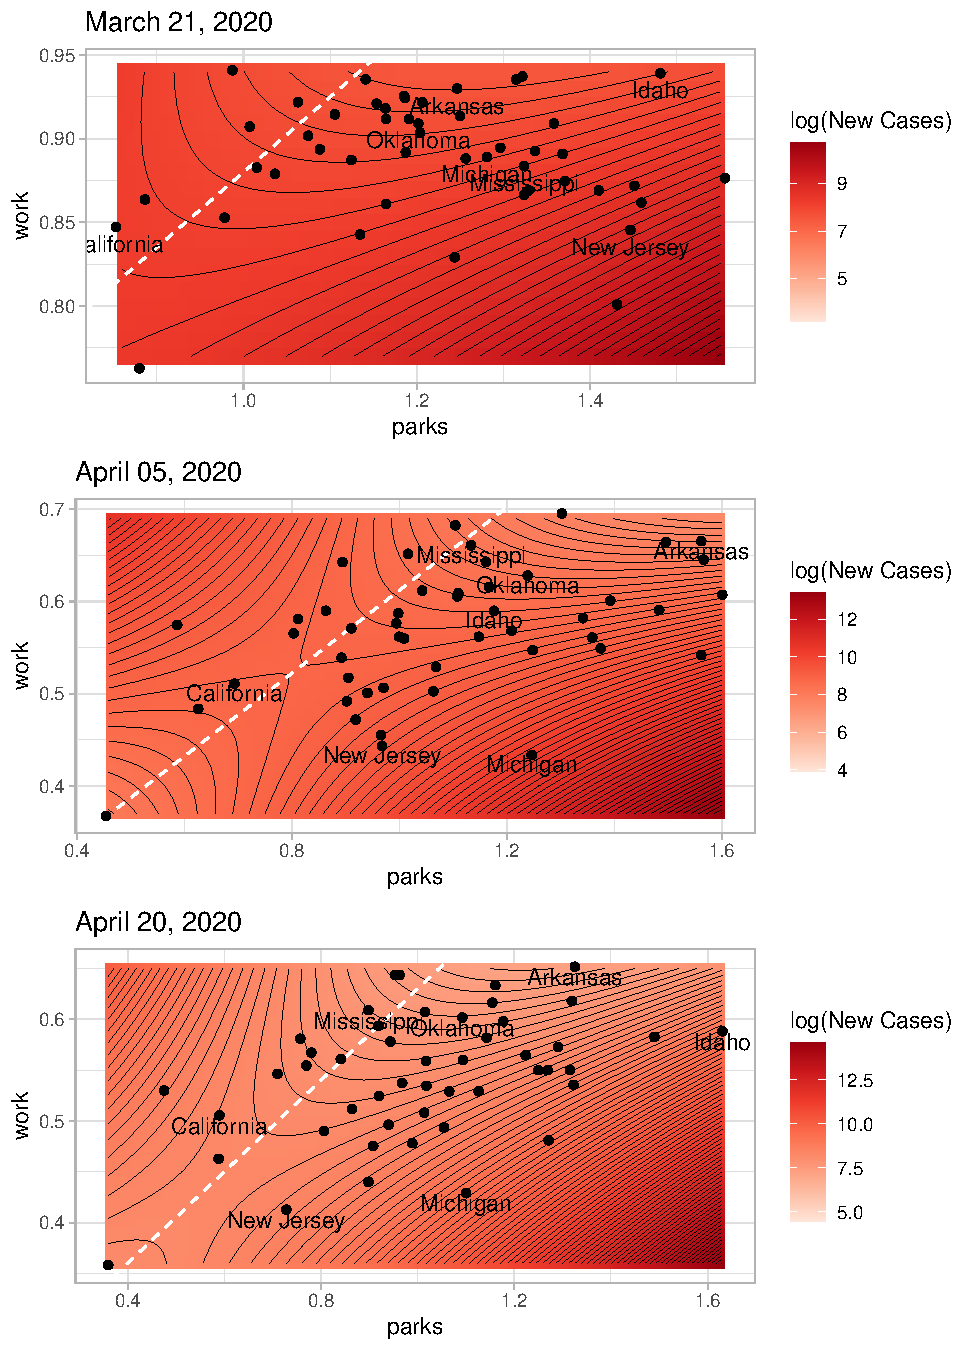
\includegraphics{Covid-19-Google-CMR-US_files/figure-latex/prediction-plots-1.pdf}
\caption{\label{fig:prediction-plots}Prediction surfaces at three points
during the pandemic according to the model; the dots are a scatterplot
of the parks- and work-related mobility indicators of the states on that
date; the white dashed line is the fold of the saddle.}
\end{figure}

The results suggest that over time the benefits of reduced work-related
mobility can be offset by parks-related mobility. For example, on March
21, New Jersey and Idaho had similar levels of park-related mobility. By
April 20, New Jersey had substantially reduced park-related mobility,
whereas Idaho's was even higher than in March. The estimated and actual
number of new cases grew in the intervening period; however, New
Jersey's growth in new cases (from March 21 to April 20) was only 894\%,
whereas Idaho's was 1030\%.

These results suggest the potential of GCMR to investigate the spread of
COVID-19, but also point at some limitations. The baseline level is not
defined in a metric that is amenable to policy development (e.g.,
person-km travelled). Without a clearer understanding of the absolute
levels of these variables, their use can suggest trends, but their
potential for applied policy analysis appears to be more limited.

\hypertarget{references}{%
\section*{References}\label{references}}
\addcontentsline{toc}{section}{References}

\hypertarget{refs}{}
\leavevmode\hypertarget{ref-Lauer2020incubation}{}%
Lauer, S.A., Grantz, K.H., Bi, Q., Jones, F.K., Zheng, Q., Meredith,
H.R., Azman, A.S., Reich, N.G., Lessler, J., 2020. The incubation period
of coronavirus disease 2019 (covid-19) from publicly reported confirmed
cases: Estimation and application. Annals of Internal Medicine.
doi:\href{https://doi.org/10.7326/m20-0504}{10.7326/m20-0504}


\end{document}


